% !TEX TS-program = pdflatex
% !TEX encoding = UTF-8 Unicode

% This is a simple template for a LaTeX document using the "article" class.
% See "book", "report", "letter" for other types of document.

\documentclass[twocolumn]{article} % use larger type; default would be 10pt

\usepackage[utf8]{inputenc} % set input encoding (not needed with XeLaTeX)

%%% Examples of Article customizations
% These packages are optional, depending whether you want the features they provide.
% See the LaTeX Companion or other references for full information.

%%% PAGE DIMENSIONS
%\usepackage{geometry} % to change the page dimensions
\usepackage[top=1in,bottom=1in, left=.9in,right=0.9in, includefoot]{geometry}
%\geometry{a4paper} % or letterpaper (US) or a5paper or....
% \geometry{margin=0.75in} % for example, change the margins to 2 inches all round
% \geometry{landscape} % set up the page for landscape
%   read geometry.pdf for detailed page layout information

\usepackage{graphicx} % support the \includegraphics command and options

% \usepackage[parfill]{parskip} % Activate to begin paragraphs with an empty line rather than an indent
%\usepackage{fourier}
%\usepackage{charter}
%\usepackage{bookman}
%\usepackage{newcent}

%\usepackage[sc]{mathpazo} % Palatino with smallcaps
%\usepackage[scaled]{helvet}
%% Helvetica, scaled 95%
%\usepackage{eulervm}
%% Euler math

\usepackage{palatino}


%%% PACKAGES
\usepackage{booktabs} % for much better looking tables
\usepackage{array} % for better arrays (eg matrices) in maths
\usepackage{paralist} % very flexible & customisable lists (eg. enumerate/itemize, etc.)
\usepackage{verbatim} % adds environment for commenting out blocks of text & for better verbatim
\usepackage{subfig} % make it possible to include more than one captioned figure/table in a single float
% These packages are all incorporated in the memoir class to one degree or another...
\usepackage[pagebackref=true, colorlinks, linkcolor=blue, citecolor=blue, urlcolor=blue] {hyperref}%
%%% HEADERS & FOOTERS
\usepackage{fancyhdr} % This should be set AFTER setting up the page geometry
\pagestyle{fancy} % options: empty , plain , fancy
\renewcommand{\headrulewidth}{0pt} % customise the layout...
\lhead{}\chead{}\rhead{}
\lfoot{}\cfoot{\thepage}\rfoot{}

%%% SECTION TITLE APPEARANCE
\usepackage{sectsty}
\allsectionsfont{\sffamily\mdseries\upshape} % (See the fntguide.pdf for font help)
% (This matches ConTeXt defaults)
\usepackage[round]{natbib}

%%% ToC (table of contents) APPEARANCE
\usepackage[nottoc,notlof,notlot]{tocbibind} % Put the bibliography in the ToC
\usepackage[titles,subfigure]{tocloft} % Alter the style of the Table of Contents
\renewcommand{\cftsecfont}{\rmfamily\mdseries\upshape}
\renewcommand{\cftsecpagefont}{\rmfamily\mdseries\upshape} % No bold!

%%% END Article customizations

%%% The "real" document content comes below...

\title{Concerning flat slab to column connection}
\author{M. A}
%\date{} % Activate to display a given date or no date (if empty),
         % otherwise the current date is printed 

\begin{document}
\maketitle
\begin{abstract}
A brief review of flat slabs and the flat slab-column connection concentrating on parameters influencing connection behavior including punching shear, shear and flexural reinforcement, connection ductility and so on is presented below.
\end{abstract}
\section{Flat plates or flat slabs }
Since early 1950s the trend toward lighter and more flexible construction configurations led to the rise of flat plates, particularly for medium- to high-rise office and residential buildings\citep{Fema2741997} although it was originally patented years earlier\citep{gasparini2002contributions,usp1909,usp1925}. Due to their beamless nature and being free of obstructions, flat slabs provide many advantages such as lower story height, better lighting and ventilation, arrangement of piping and wiring, more clear space in addition to architectural flexibility and easier formwork in construction. 

Despite the architectural charm this system doesn't have a well established seismic reputation and due to it's vulnerability to seismic loads it's behavior is normally a matter of concern\citep{HosahalliSomaprasadR1994SVoF,Derecho2001} which doesn't make one wonder why \cite{aci31819} applies the lowest inertia moment factor ($0.25$) to flat slabs and flat plates for elastic analysis at factored load levels. Research on two-way flat slabs with drop panels indicates that in this particular case they have similar behavior to flat plates\citep{odello1967behavior}. It's notable that detailing requirements for two-way slabs without beams as mentioned earlier for flat plates in \citet[Chapter 21]{aci31895} appear only in the section relating to areas of moderated seismic risk which in turn suggests that \cite{aci31895} considers the use of flat plates as acceptable components of the lateral-load-resisting system only for areas of moderate seismicity\citep{Derecho2001}. Punching shear failure at slab-column connection for this system because of its brittle nature and potential in triggering progressive collapse may lead to catastrophic losses as evidenced in the past\citep{king2004,PARK2012119}.
    
Ductile detailing of all structural connections, including also for those with only gravity load has become a key concept that was learned as a result of failures observed during the 1971 San Fernando Valley Earthquake. Slab-column connections in a flat plate structure though only gravity loaded must maintain load bearing capacity at maximum lateral displacement allowed by the lateral load bearing system during which there is chance of brittle failure modes like slab punching shear taking place if this displacement is not absorbed by slab-column interfaces\citep{DoD2016}. This mode of failure could occur with little or no warning signs that has resulted in the progressive collapse of this type of structures as in the 1985 Mexico City earthquake in which 91 flat plate buildings collapsed and 44 others were severely damaged due to punching failure\citep{ghali2000stud}. Notably flat slab performance remained poor in the 2017 Mexico City earthquake also\citep{insufi2020}. Although punching failure occurs during the earlier stages of construction too, when concrete has yet to harness reliable strength to resist shear effects\citep{gardner2011}. 


The Iranian code of standard practice for seismic design of buildings\citep[Section 3-3-5-5]{28002014} restricts the use of flat slabs either with or without drop panels to buildings at maximum 3 stories or 10m tall. Whereas in \cite{aci31819} slab-column frames without beams are at most accounted as intermediate moment frames and per \citet[Section R18.2]{aci31819} are not permitted as part of seismic-force-resisting systems for structures assigned to Seismic design classification (SDC) D, E, or F and are only allowed as a gravity or secondary system where shear walls form the seismic or lateral force resisting system (SFRS or LFRS). The reasoning for this simply put by \citet[Chapter 7]{JointACI-ASCECommittee4212015} is that these frames cannot meet the detail requirements for the level of energy dissipation and ductility demanded for special moment frames. Even when an independent lateral-force-resisting system is provided \cite{JointACI-ASCECommittee4212015} suggests that flat plate-column connections should be designed to accommodate the moments and shear forces associated with the displacements or story drifts during earthquakes. Thus all members in slab-column frames not designated as part of the SFRS should be designed to support gravity loads while subjected to design displacements.  

During the recent decades various laboratory tests concerning flat slabs have been carried out which are distinguishable in three specimen size classes as \begin{itemize}\item isolated slab-connections, \item complete single floors, \item and complete frames least two stories tall. \end{itemize}
Numerous research has been done as presented herein studying isolated slab-column connections under combined gravity and lateral loading\citep{dovich2005,drakatos2016,hawkins1979,hueste2007,kang2006,megally2000,pan1989,robertson2002,setiawan2019,tian2008,andre2016} while fewer have been in the form of size scaled floors tested under cyclic loads\citep{hwang1993,hwang2000,rha2014} and only four consisted of complete buildings\citep{coronelli2021,fick2017,moehle1984,kang2004}. \cite{coronelli2020} provides an state of the art review of these larger scale tests and an introduction to the ``Slab STRESS'' research program reported by \cite{coronelli2021} in which a full-scale flat slab specimen is tested. \cite{coronelli2021} carried out seismic tests for service and ultimate actions using pseudodynamic technique with virtual walls in which the flat slab frame was the secondary element as suggested by \cite{asce4117,fema356}\footnote{\cite{asce4117} classifies building components as either primary or secondary in respect to their role in resisting the seismic forces and whether their failure or degradation would compromise building lateral stability, thus secondary elements would be any building structural element whose purpose is to support gravity loads. \cite{asce4117} requires that both primary and secondary components be evaluated to confirm their seismic force and deformations do not behave inconsistently with the selected performance level therefore the standard also states that where a component intended in the original building design as primary is deformed beyond the point where it can be relied to resist earthquake effects, the secondary designation may be used.}. 

Moment and crack distribution and redistribution in multi bay slab column frames due to nonlinear behavior and progressive deterioration of joints are major draw backs for isolated connection subassemblies which might fail at providing accurate boundary conditions\citep{einpaul2015,einpaul2016}. \cite{einpaul2015} investigated moment redistribution between hogging and sagging moments and compressive membrane action influence on conventional isolated connection experiments suggesting that the punching capacity of continuous slabs with low amounts of flexural reinforcement on the interior column regions may be underestimated in the codes of practice. Note that there are plenty of tests on internal slab-column connection specimens while results for edge or corner columns are less frequent. 


\subsection{Punching shear}
Early foundations for punching shear design was laid in \cite{talbot1913reinforced} though through examination was not carried out until much later \citep{elstner1956shearing,moe1961} without moment application that are reviewed in detail by \cite{ghoreishi2013review,yang2011data,hamada2008evaluation}. 
\begin{figure}\centering
    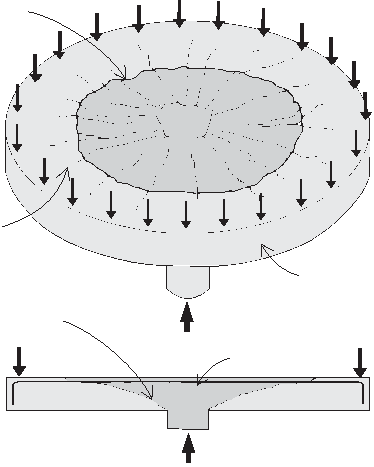
\includegraphics[width=\columnwidth]{Figures/tikzout/b16if1.pdf}\caption{Isolated interior flat slab-column connection region and typical punching shear failure surface, adapted from \cite{bompa2016b}: a) Isometric view; b) Section view.}\label{b16if1}
    \end{figure}
On the other hand \cite{kinnunen1960} proposed that flat slab punching strength is related to slab flexural deformations in the column vicinity that was further improved by \cite{shehata1989punching,broms1990}.

Column connection region behavior in reinforced concrete elements is characterized by flexural crack developments at incipient loading stages (\ref{b16if1}a and \ref{b16if2}c). 

Typically with low reinforcement ratios at an ultimate state these cracks may govern connection behavior leading to a potential yield of longitudinal reinforcement (\ref{b16if3}c) \citep{hallgren1996punching}.  If flexural behavior doesn't govern and with reinforcement stresses nigh on bar yield stress, flexural cracks would propagate into shear cracks leading to a failure mode defined as flexural punching\citep{fib2001}.

    \begin{figure}\centering
        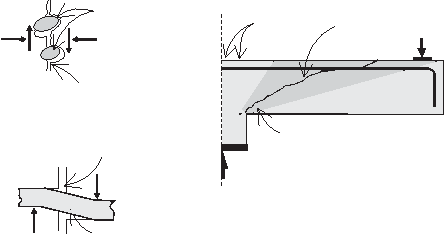
\includegraphics[width=\columnwidth]{Figures/tikzout/b16if2.pdf}\caption{Slab-column connection cracks, adapted from \cite{bompa2016b}: a) Aggregate interlock; b) Dowel action; c) Compression field.}\label{b16if2}
        \end{figure}

In case of high reinforcement ratios the slab behaves stiffer with reinforcements bearing lower stresses and higher stresses concentrated in the inclined concrete compression zone developed near the column (\ref{b16if3}a)\citep{hallgren1996punching}. Punching shear failure is described as the development of a diagonal crack with variable inclination starting from the column face on the slab compression side and ending at the slab tension face resulting in the dislocation of a conical body of concrete slab (\ref{b16if1}) \citep{regan1986}.

\begin{figure}\centering
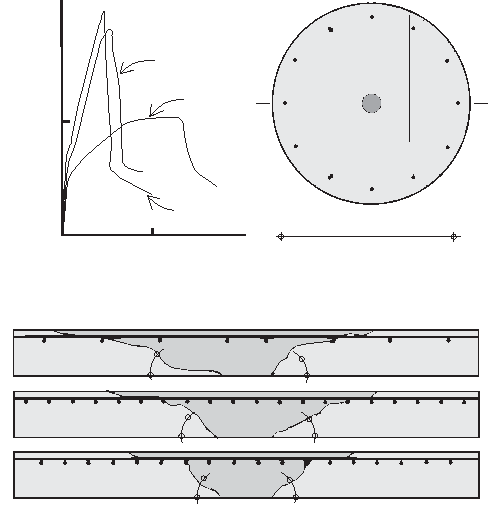
\includegraphics[width=\columnwidth]{Figures/tikzout/b16if3.pdf}\caption{Test results (HSC0, HSC4, HSC9) carried out by \cite{hallgren1996punching},  adapted from \cite{bompa2016b}: a) Structural response; b) In-plane geometrical configuration; c) Sectional view of saw cuts.}\label{b16if3}
\end{figure}
\begin{figure}\centering
    \includegraphics[width=\columnwidth]{Figures/tikzout/fr181451.pdf}\caption{Slab shear reinforcement requirement criteria, recreated from \cite{aci31819}.}\label{fr181451}
    \end{figure}
Typically in concrete members shear is carried by \begin{itemize}\item the interlock and frictional resistance of the cracked interface aggregates against crack slip and growth\citep{walraven1981}, \item dowel bar shearing\citep{dei1987,dei1992,ince2007,paulay1974,taylor1970}, \item transmission through the concrete section compression zone\citep{chana1987}, \item and residual stress transfer through the crack tip(\ref{b16if2} a,b)
\end{itemize}
Stress distribution in the column-slab connection region governs punching shear crack inclination angle and the slab punching shear strength is governed by the amount of shear carried or resisted by the cracked interface. The inclination angle and punching shear capacity depend on member geometry\footnote{Depth, slenderness, column dimensions to slab thickness ratio.} and structural parameters\footnote{Material strengths, aggregate properties, reinforcement layout and so on.}. As the inclination angle reduces and the cracked interface parallels the slab faces further, the interlocking surface widens, also more bars get involved in dowel action thus larger amounts of shear are transferred. \cite{inacio2015} carried out an experimental study(\ref{i2015f1}) over high strength concrete (HSC) flat slabs without shear reinforcement testing four specimens, one of which was built with normal strength concrete (NSC). Significant load capacity increase compared to the reference NSC specimen was observed and the results furthermore indicate that longitudinal reinforcement increase had a positive influence on punching shear capacity\citep{inacio2015}. \cite{emam1997seismic,marzouk2001cyclic} studied high strength and light weight concrete application in flat slabs. \cite{kadhim2021} showed punching shear capacity improvement with ultra-high performance concrete (UHPC) use in flat slabs without shear reinforcement through a nonlinear finite element procedure implementing \cite{abaqus} verified against \cite{saleem2011,zohrevand2015punching}. 
\begin{figure}\centering
    \includegraphics[width=\columnwidth]{Figures/i2015f1.pdf}\caption{Test setup\citep{inacio2015}.}\label{i2015f1}
    \end{figure}
    
\cite{qi2021} carried out concentrated load tests on eight similar flat slab specimens in three groups to study UHPC depth and area influence on flat slab punching shear behavior the application of which at full depth(\ref{q2021f1}) over the critical section area transformed the brittle punching shear failure mode into a ductile punching shear-flexure one while limited depth UHPC application over this area ended in brittle failure. 
\begin{figure}\centering
    \includegraphics[width=\columnwidth]{Figures/q2021f1.pdf}\caption{Test setup\citep{qi2021}.}\label{q2021f1}
    \end{figure}
    
\cite{ramos2022} tried high-performance fiber reinforced concrete (HPFRC) application in slab-column connection vicinity as a substitute for shear reinforcement with four specimens under combined gravity and horizontal reversed cyclic loading in which connection drift capacity substantially improved compared to reference specimens and the HPFRC reinforced specimens performed better than specimens with HSC. \cite{ricker2017} carried out ten punching tests on slab-column connections with double-headed studs as shear reinforcement nine of which had fiber reinforced UHPC units in the slab-column connection compression zone(\ref{r2017f1}) that reached significantly higher failure loads compared to normal specimens. 
\begin{figure}\centering
    \includegraphics[width=\columnwidth]{Figures/r2017f1.pdf}\caption{Layout of flexural reinforcement and double-headed studs for test specimen DUHPC2\citep{ricker2017}.}\label{r2017f1}
    \end{figure}
    \begin{figure*}\centering
        \includegraphics[width=\textwidth]{Figures/r2017f2.pdf}\caption{UHPC units\citep{ricker2017}.}\label{r2017f2}
        \end{figure*}
Another concrete behavior improvement approach for slab-column joints has been introduced through the use of steel fiber additives in the concrete mix as studied by \cite{gouveia2018,gouveia2014,ABDELRAHMAN2018272,ju2015} that improves a plethora of structural characteristics in addition to punching shear strength including load bearing and flexural capacities along with structural stiffness and connection ductility. 
\section{Slab-column connection}
Tests on slab-column connections subjected to reversed cyclic loading\citep{carpenter1973design,symonds1976slab} indicate that ductility of flat slab-column connections can be significantly increased through the use of stirrups enclosing bands of flexural slab reinforcement passing through the columns\footnote{Such shear-reinforced bands would essentially function as shallow beams connecting the columns.}. \citep{Robertson2006} observed that an increase in the flexural stiffness of a slab-column connection induces a higher shear demand. Also \citep{Robertson2006} concluded that connections with increased slab flexural reinforcement will support greater lateral loads, but the increased eccentric shear transfer may result in premature punching shear failure. However tests on interior column-to-slab connections with lightly reinforced slabs with and without shear reinforcement \citep{peiris2012flexural,hawkins2017effect,bayrak2009two,muttoni2008punching,dam2017behavior,muttoni2008punching} have shown that yielding of slab flexural tension reinforcement in the vicinity of the column or loaded area leads to increased local rotations and opening of any inclined crack existing within the slab. In such cases, sliding along the inclined crack can cause a flexure-driven punching failure at a shear force less than the strength calculated by the two-way shear equations of \citet[Table 22.6.5.2]{aci31819} (\ref{eqt22652}) for slabs without shear reinforcement and less than the strength calculated in accordance with \citet[Section 22.6.6.3]{aci31819} for slabs with shear reinforcement. 

Tests of slabs with flexural reinforcement less than $A_{s,\min{}}$ have shown that shear reinforcement does not increase the punching shear strength\citep{aci31819}. However, shear reinforcement may increase plastic rotations prior to the flexure-driven punching failure\citep{peiris2012flexural}. Whereas \cite{megally2000punching,kang2006,robertson2002cyclic} argue that connection ductility will increase with shear reinforcement application in slab-column connections. This is sound mainly because slab connection will yield or fail in flexure prior to punching shear. \cite{kang2006,megally2000punching,robertson1991,robertson1993,anggadjaja2008} showed that gravity load strongly influences flat slab-column connection lateral ductility and with gravity load increase connection lateral displacement capacity decreases that was also observed in reviewed test data by \cite{aci4212010} to assess gravity load effect on lateral drift capacity for interior flat plate-column connection specimens with and without shear reinforcement. Also tests have shown that beam-column joints laterally supported on four sides by beams of approximately equal depth exhibit superior behavior compared to joints without all four faces confined by beams under reversed cyclic loading\citep{hanson1967seismic}. 
\subsection{Shear reinforcement}
Provisions for shear reinforcement at slab-column connections for non-SFRS members were adapted in \cite{aci31805} to reduce slab punching shear failure likelihood. \citet[Section 18.14.5]{aci31819} states for nonprestressed slabs that design story drift ratio is limited to the following
\begin{equation}\label{eqdr}
\frac{\Delta_x}{\mathbf{h_{sx}}}\ge\mathbf{0.035-0.05\frac{v_{uv}}{\phi v_c}}
\end{equation}
presented in \ref{fr181451}.
If the drift ratio exceeds this amount(\ref{eqdr}) thus slab shear reinforcements either stirrups or headed studs should be provided at any slab critical section considering that $\mathbf{v_{uv}}$ is evaluated with load combinations including earthquake effect $\mathbf{E}$ and $\Delta_x/\mathbf{h_{sx}}$\footnote{$\mathbf{v_{uv}/(\phi v_c)}$ is otherwise known as the ratio between the acting vertical shear force and the punching shear resistance or Gravity shear ratio (GSR) in the literature. Larger GSRs imply lower frame or structure horizontal deformation or drift capacity and are possible with shear reinforcement\citep{gouveia2019}.} is the greater of values for adjacent stories above and below the slab-column connection while $\mathbf{v_c}$ is evaluated as below. 
\begin{equation}\label{eqt22652}
\mathbf{v_c} = \min{\left[\begin{array}{c}
1\\
1/2+{1}/{\beta}\\
1/2+{\alpha_sd}/{4b_o}\\
\end{array}\right]}
\frac{\lambda_s\lambda\sqrt{f'_c}}{3}
\end{equation}
where $\beta$ is the ratio of long to short column sides or supporting element, $\mathbf{\alpha_s}$ is the factor accounting for connection location, $\mathbf{d}$ is the slab effective depth, $\mathbf{\lambda_s}$ is the size effect factor, and regardless of shear reinforcement the critical section perimeter $\mathbf{b_o}$ is at least $\mathbf{d/2}$ away from column edges or changes in slab thickness minimizing $\mathbf{b_o}$ while with shear reinforcement an extra critical section $\mathbf{d/2}$ away from the outermost peripheral line of shear reinforcement considering the shape should be a polygon minimizing $\mathbf{b_o}$ is added\footnote{There will be two critical sections for shear reinforced sections.}, 
\begin{equation}\nonumber\begin{array}{rl}
\lambda_s =& \sqrt{{2}/({1+0.004d})}\ge1, \lambda = 1\\
\alpha_s =&\left\{\begin{array}{ll}40&\mathrm{interior}\\ 30& \mathrm{edge}\\20&\mathrm{corner}\end{array}\right.\,\mathrm{columns}
\end{array}
\end{equation}
Development of \ref{eqt22652} is reviewed in \cite{bayrak2009two}. Also note that most of the existing research on punching shear are based on test results from reinforced concrete column and slab specimens.



\cite{megally2002,moehle1996,kang2006,kang2007} identified the likelihood of punching shear failure about the slab critical section without moment transfer considering story drift ratio and shear stress $\mathbf{v_{uv}}$ due to gravity loads and the vertical component of earthquake loads therefore no induced moment calculations would be necessary. \cite{megally2000,kang2009nonlinear,moreno2008punching,song2012effective,kruger1998punching,krueger1999influence} found that moment presence significantly decreased slab punching shear resistance  that is in line with earlier findings \citep{hawkins1974,islam1976}. The above mentioned requirement (\ref{fr181451}) can also be satisfied by increasing slab thickness, changing the design to reduce story drift ratio, or a combination of all of the above. 
    
The shear reinforcement in the slab critical section should provide $\mathbf{v_s\ge0.29\sqrt{f'_c}}$ extending at least four times the slab thickness from the support face adjacent to it. In case the above requirements are not met for two-way slabs that are designated as part of SFRS \citet[Section 18.4.5.8]{aci31819} states that two-way shear stress caused by factored gravity loads without moment transfer should not exceed $\mathbf{0.4\phi v_c}$ beyond which nonprestressed slab-column connections in laboratory tests by \cite{pan1989} exhibited reduced lateral displacement ductility. 
\begin{figure}\centering
    \includegraphics[width=\columnwidth]{Figures/akt1.pdf}\caption{Model column geometries\citep{akinpelu2023}.}\label{akt1}
    \end{figure}

Variety in shear reinforcement lies partly on a practical point, when various construction limitations arise such as difficulties in proper bar placement or improper stirrup configurations after slab reinforcement is done or even shear head sections barring essential reinforcement in the column and slab considering the \cite{ACI31814} requirements such as uninterrupted inserts.

\cite{moe1961} tried to increase column effective size placing steel plates with a certain overhang as illustrated in \ref{h74f1}(a) over the column and was successful at achieving increased capacity noting that shear was concentrated on plate corners. \cite{akinpelu2023} carried out a numerical study of column shape effect on flat slab punching shear behavior implementing the finite element package ABAQUS\citep{abaqus} in which the authors tried $\mathrm{L}$, $\mathrm{T}$ and $\mathrm{+}$ column geometries maintaining the column area and perimeter also introducing damage plasticity into the model(\ref{akt1}). The simulation results of \cite{akinpelu2023} showed that  the $\mathrm{+}$ geometry renders a larger column effective size and thus behaves better than others in comparison to rectangular sections\citep{akinpelu2023}. \cite{hawkins1968} studied the bearing strength of these steel plates and proposed a plate thickness formula to provide maximum increase in column effective size without disadvantageous corner effects.

\subsubsection{Shearheads}
    \begin{figure}\centering
        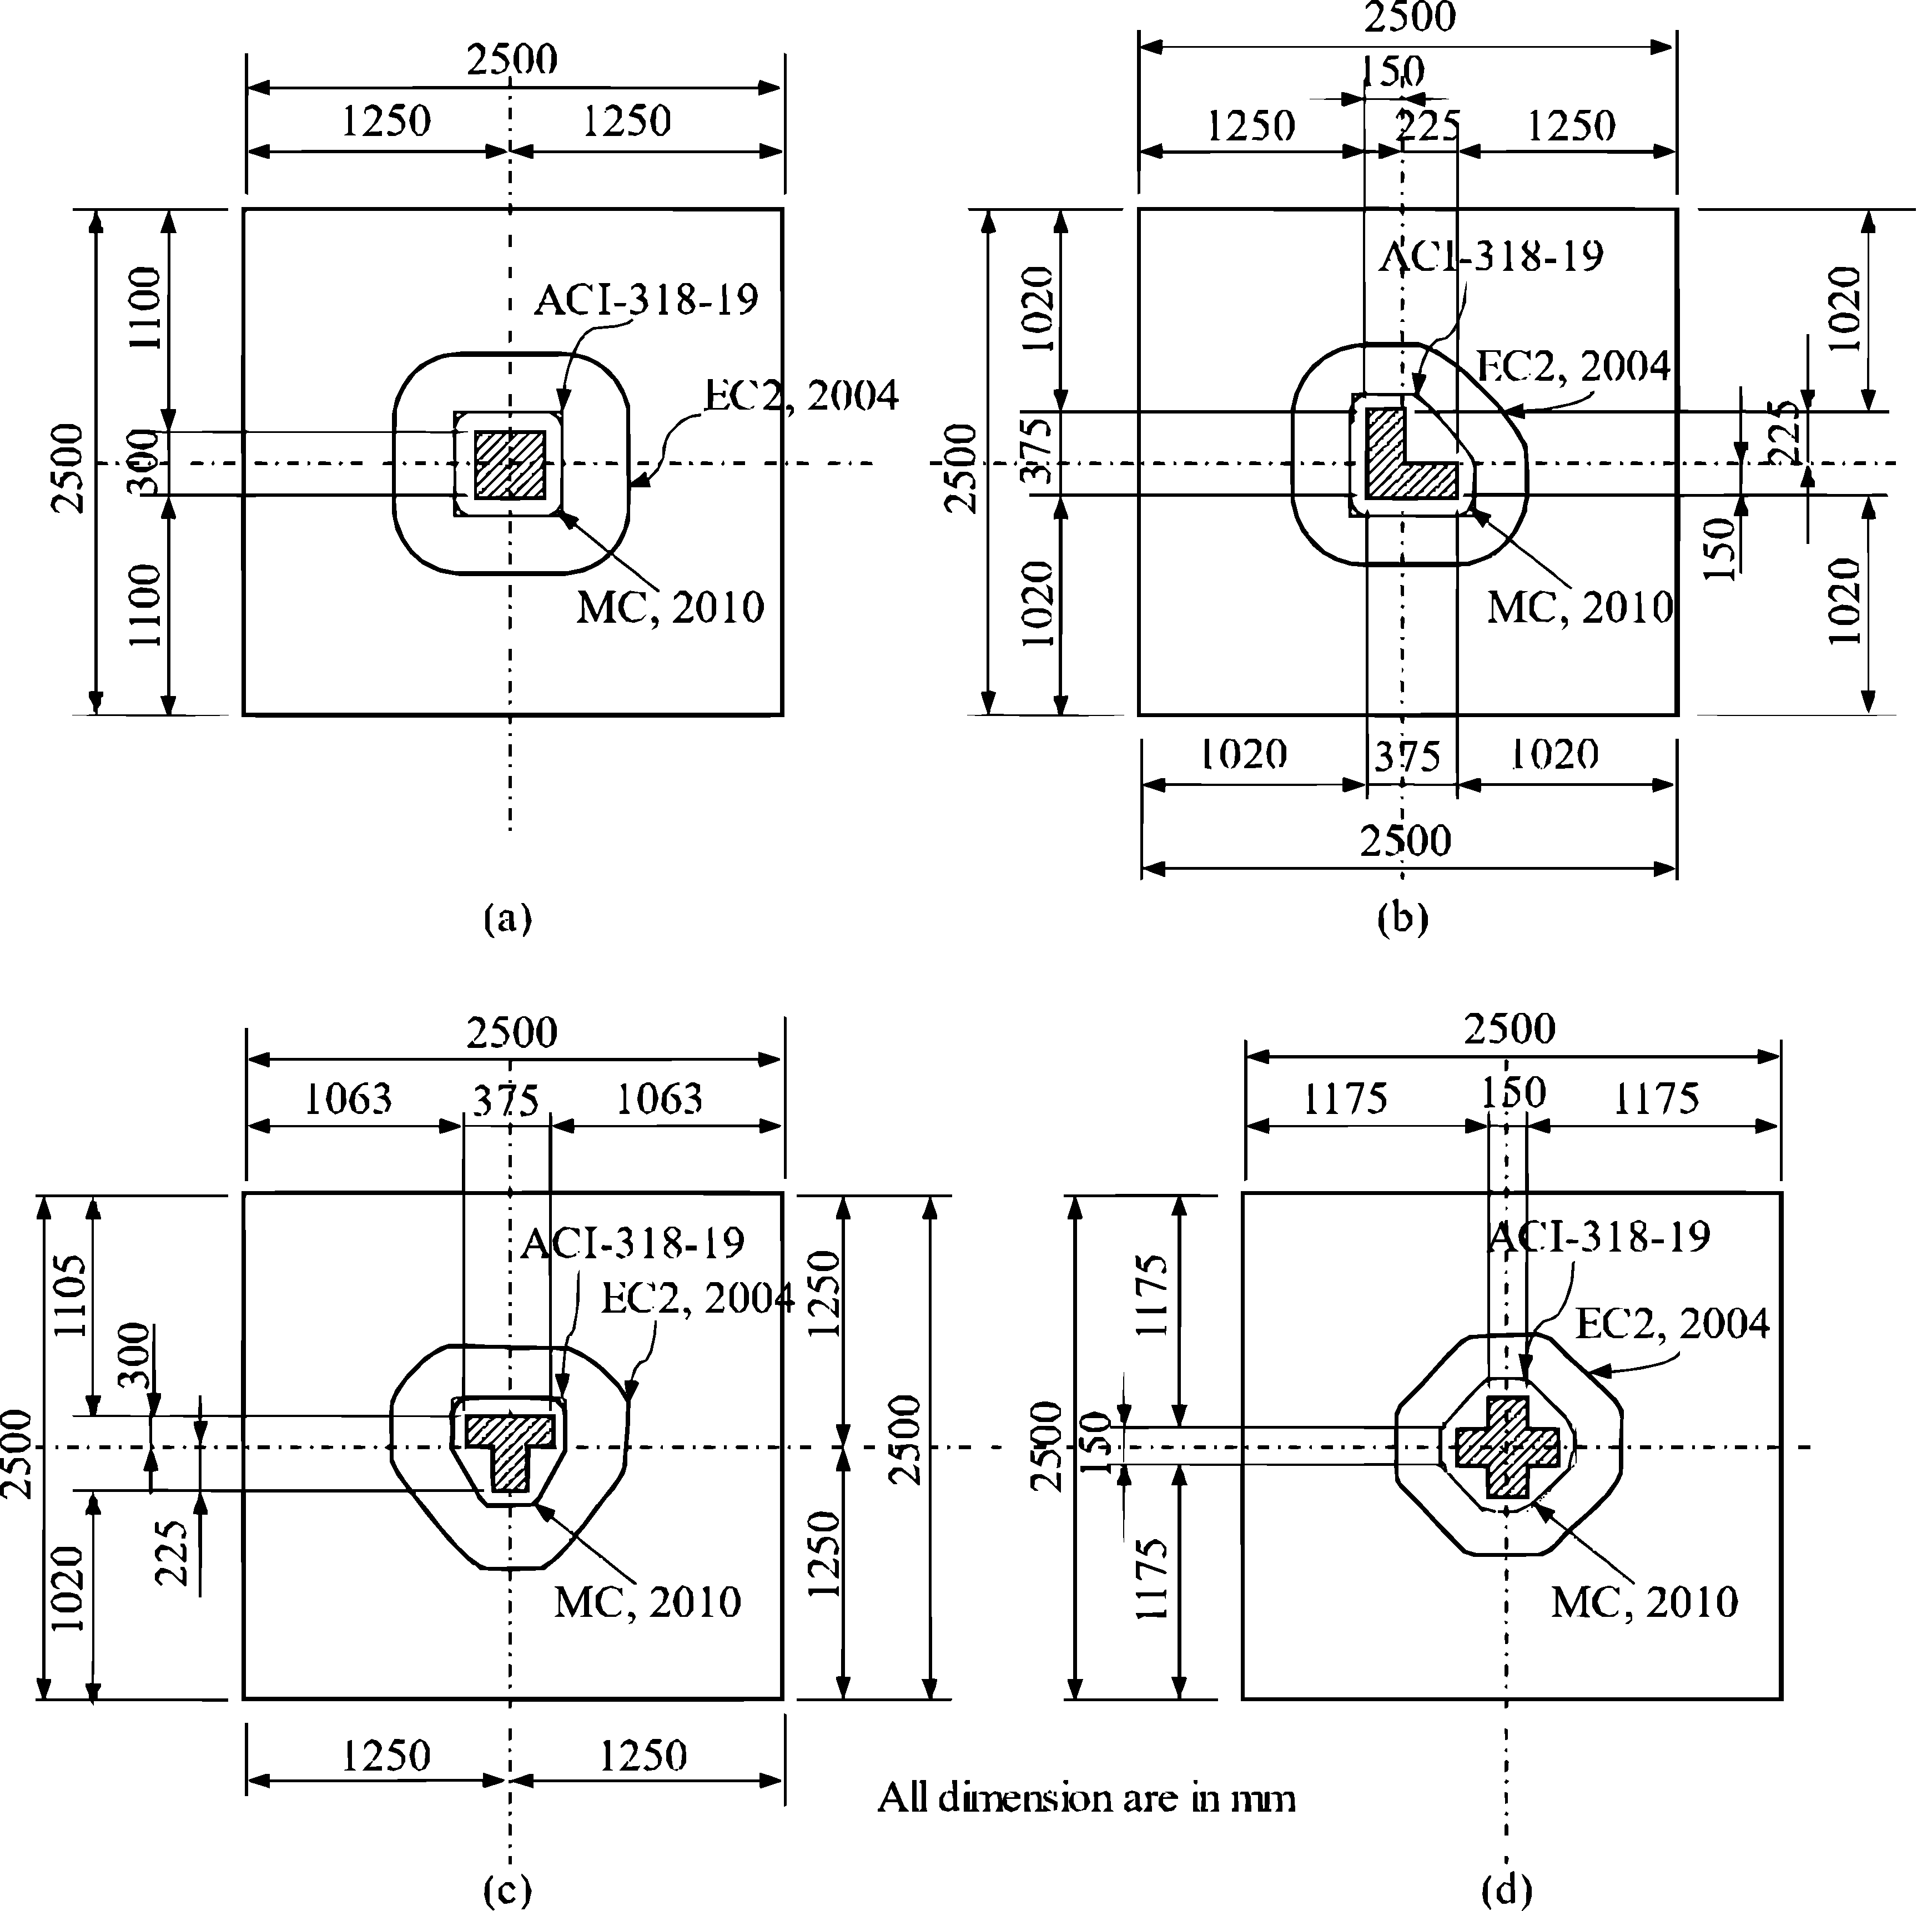
\includegraphics[width=\columnwidth]{Figures/akf3.pdf}\caption{Layouts of modelled flat slabs showing critical sections as per various code provisions, adopted from \citep{akinpelu2023}; a) Square column; b) $\mathrm{L}$; c) $\mathrm{T}$; d) $\mathrm{+}$.}\label{akf3}
        \end{figure}
\begin{figure}\centering

\includegraphics[width=\columnwidth]{Figures/tikzout/h74f1m.pdf}
\caption{Shear reinforcements\citep{hawkins1974a}; a) Steel plate\citep{moe1961}; b) Channel sections\citep{hawkins1974}; c) $\mathrm{I}$ sections\citep{hawkins1974}; d) Collar\citep{tasker1963}; e) Shearhead-SH, cage; f) Shearhead cage-SH; g,h) Bent bars-B; i) Bent radial bars-BR; j) Radial stirrups-RS; k) Vertical stirrups-VS; l) Inclined stirrups-IS; m) Close stirrups-CS, Radial-CSR, Tangential-CST; n) U-shaped stirrups-US; o) Beam stirrups-BS.}\label{h74f1}
\end{figure}

Shearheads are another type of shear reinforcement that despite being originally introduced in \cite{wheeler1936} are seldom used in current practice so their design provisions have been omitted in \cite{aci31819} and may be designed following \cite{ACI31814} provisions. Design criteria in \cite{aci31871} were developed based on shear forces in \cite{hawkins1974,corley1968} who performed 21 tests, 16 of which were with cruciform grillages of $\mathrm{I}$ and $\mathrm{C}$ steel sections complementing \cite{corley1968,hawkins1974}(\ref{h74f1} b,c) and the approach has been maintained up to \cite{ACI31814}. Results from \cite{hawkins1974a} contrasted with \cite{aci31871} provisions and \cite{hawkins1974} also showed that after cracking in the slab around the connection the subsequent shear forces applied are carried by the shearhead module while failure initiates either through punching along the shearhead perimeter or reaching the shearhead flexural capacity. Commentary on \citet[Section 22.6.9]{ACI31814} suggests that a minimum flexural strength should be provided to ensure slab shear strength is reached before shearhead flexural strength is exceeded. The above mentioned shearheads (\ref{h74f1} b,c) increased slab shear capacity as shearhead arm length grew thus \cite{corley1968,hawkins1974} introduced the critical sections and equations for column face moment and shear illustrated in \ref{fr2269814}. These results were adopted by \cite{Al-hamd2018} who proposed two new shearhead designs (\ref{ahf5}) based on nine laboratory tests with eccentrically loaded specimens with an offset corbel (\ref{ahf4}) similar to \cite{kruger1998} followed by a numerical study of connection behavior. Load and moment in the manner described by \cite{kruger1998,Al-hamd2018} is quite advantageous compared to \cite{ghali2000stud,kang2009nonlinear,moreno2008punching,song2012effective,hawkins1974,islam1976} who produced moments by applying a lateral load to one of the column sides. While reporting results from testing shearhead systems to improve steel column-flat slab connection ductility under cyclic loads \cite{EDER2012239} made a similar argument to the above pointing out that slab behavior is controlled by shearhead stiffness and high connection strength and ductility are realizable when using partially integrated shearheads if dissipative elements are designed to yield in shear first. 
\begin{figure}\centering
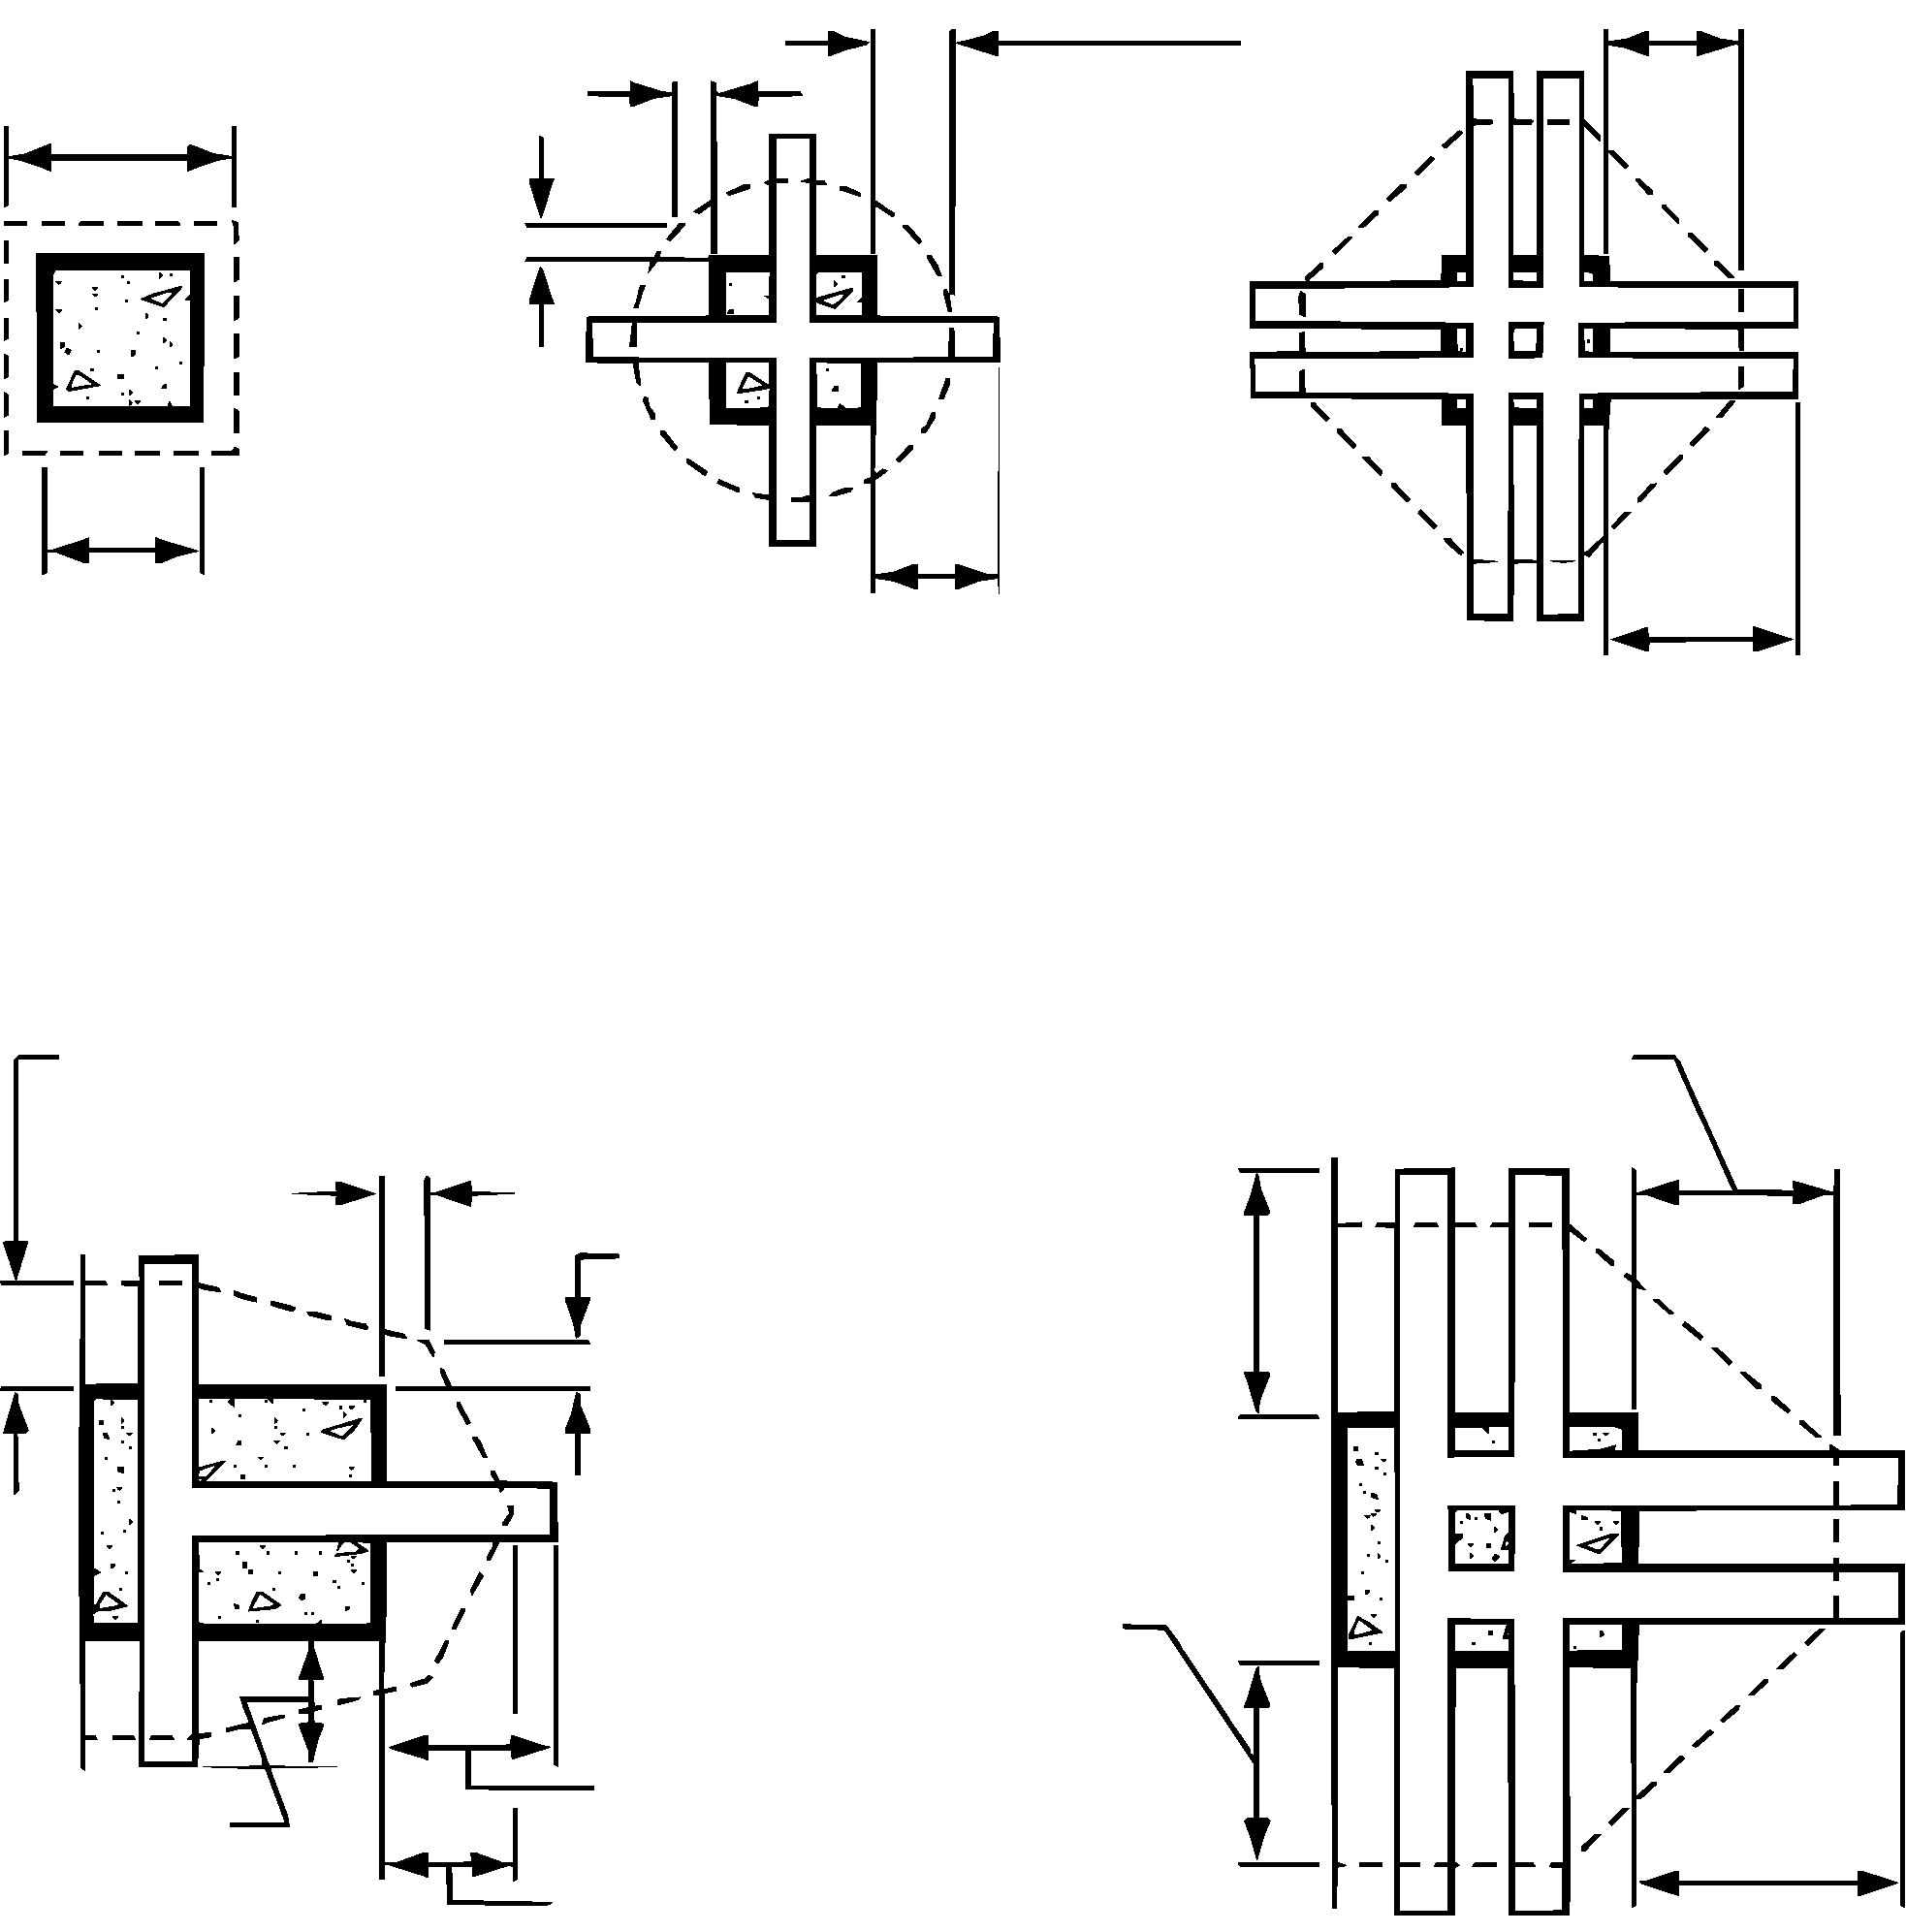
\includegraphics[width=\columnwidth]{Figures/tikzout/fr2269814.pdf}
\caption{Flat slab shear critical sections with and without shearhead adapted from \cite{ACI31814}; a,b,c) Interior columns same as \cite{hawkins1974a}; d,e) Edge columns.}\label{fr2269814}
\end{figure}
Steel columns and flat slabs are generally connected with steel inserts welded to the column and then integrated into the slab\footnote{More on this in \ref{cft}.}.

Shearhead response in accord with \ref{fr2269814} is ensured by anchoring the shearhead steel section flanges within the slab compression zone based of which \cite{aci31871} requires having the compressions flange within $0.3\mathbf{d}$ of the slab compression surface. \cite{godycki1984} showed embedment length on ultimate connection capacity for flat slabs with cruciform or $+$ shearheads under eccentric loading.

\begin{figure}\centering
\includegraphics[width=\columnwidth]{Figures/tikzout/ahf5.pdf}
\caption{Proposed shearhead layouts by \cite{Al-hamd2018}; a) G2; b) G3. }\label{ahf5}
\end{figure}
\begin{figure}\centering
\includegraphics[width=\columnwidth]{Figures/ahf4.pdf}
\caption{Tested slab geometry with offset corbel by \cite{Al-hamd2018} (all dimensions in mm).}\label{ahf4}
\end{figure}

\cite{bompa2015} proposed a method for punching shear evaluation of reinforced concrete flat slab-column connections without shear reinforcement. Having studied shear behavior of beam to steel column assemblages\citep{bompa2016b} with a series of 5 large scale tests with shearheads or arms welded to the steel column and embeded in reinforced concrete beams, \cite{Bompa2016a} carried out six large scale tests and developed an analytical model for steel column-flat slab connection with shearheads(\ref{bf2}) that showcased the positive influence of continuity plates connecting the shearheads. The shearheads were welded to the steel column and fully embedded in the slab while in the 6 test specimens the embedment length, slab thickness and shearhead cross section were maintained whereas shearhead assemblage configuration, flexural reinforcement ratio and transverse reinforcement contributions varied. \cite{bompa2020} Carried out a a thorough three-dimensional nonlinear numerical and parametric analysis implementing the concrete damage plasticity models validated against experimental results from three test series\citep{guandalini2009punching,chana1996,hawkins1974} and proposed analytical models for connection rotational response as well as the ultimate strength of reinforced concrete slab systems provided with fully embedded shearheads(\ref{b2020f2}). 
\begin{figure}\centering
    \includegraphics[width=\columnwidth]{Figures/bf2.pdf}
    \caption{Specimen arrangement \cite{Bompa2016a}; a) Longitudinal reinforcement layout; b) I-I cross-sectional view; c) transverse reinforcement layout; d) II-II cross-sectional view from transverse reinforcement; e) Shearhead details, without continuity plate on the left and with continuity plate on the right.}
    \label{bf2}
    \end{figure}
\begin{figure}\centering
    \includegraphics[width=\columnwidth]{Figures/b2020f2.pdf}
    \caption{Schematic representation of specimens numerically studied in \cite{bompa2020}; a) Full scale specimens PG1, PG2b, PG5, PG10, PG11; b) Half scale specimens PG6, PG7, PG8, PG9; c) Double scale specimen PG3 from \cite{guandalini2009punching}; d) FSSH series; e) SH series from \cite{chana1996}; f) A and B series \citep{hawkins1974}; Cruciform shear-heads made of g) Welded back-to-back channel or I sections (CRH); h) Two pairs of channels at the support region (CTP) shearheads; i) Closed-box shearheads (CBX).}
    \label{b2020f2}
    \end{figure}
\cite{eder2010} validated a nonlinear finite element model against a large-scale reinforced concrete flat slab without shear reinforcement that failed in punching and subsequently carried out a parametric analysis of key parameters. These authors modelled a large scale hybrid reinforced concrete flat slab specimen tested at the London Imperial College with a steel column and \cite{aci31808} type steel shearhead as well. Their analysis suggests that loads are principally transferred into the shearhead arm tips if the failure surface lies outside shearhead arm length while a more uniform load transfer into these arms would occur if the failure surface lies inside. \cite{EDER20111164} presented a novel partially integrated shearhead detail(\ref{e2011f3}) with a gap around the tubular steel column(\ref{e2011f4}) to enable shearhead yield in the shearhead prior to slab punching shear and compared it with the typical \cite{aci31808} shearhead presenting test results from four large-scale specimens and numerical analysis under gravity and cyclic lateral loadings following which \cite{EDER2012239} further studied the inelastic performance and design of this novel ductile steel shearhead with additional u-bars under these loads. \cite{EDER2012239} notes that I section shear arms perform better than closed box sections due to improved composite action with the slab and also suggests anchoring of the shear arms to the slab through end plates or otherwise to further resist the siginificant axial forces which arise as a result of geometric nonlinearity. 
    \begin{figure}\centering
    \includegraphics[width=\columnwidth]{Figures/e2011f3.pdf}
    \caption{Specimen reinforcement layouts in \cite{EDER20111164}.}
    \label{e2011f3}
    \end{figure}
\begin{figure}\centering
    \includegraphics[width=\columnwidth]{Figures/e2011f4.pdf}
    \caption{Shearhead detail proposed in \cite{EDER20111164}.}
    \label{e2011f4}
    \end{figure}
\begin{figure}\centering
    \includegraphics[width=\columnwidth]{Figures/e2012f1.pdf}
    \caption{Test rig used for large-scale tests\citep{EDER2012239}.}
    \label{e2012f1}
    \end{figure}

\subsubsection{Bent bars and stirrups}
\cite{bavzant1987size} improved understanding of member size effect on slab behavior with large scale specimens and proposal of a design formula. Following an experimental program \cite{shehata1989punching} presented a mechanical model to estimate punching shear resistance of axisymmetric slabs under concentric loads.  In order to analyse punching shear resistance of flat slabs with shear reinforcement \cite{gomes1999} proposed an analytical model based on \cite{kinnunen1960,shehata1989punching} validated on 12 full scale test specimens. \cite{birkle2008} focused on the influence of slab thickness while \cite{beutel2002} studied anchorage effect on shear reinforcement effectiveness over the shear punching critical section. Detailed investigations by \cite{guandalini2009punching,muttoni2008punching} resulted in a analytical model of punching shear strength as a function of slab rotation that formed the basis for \cite{mc2010} as well. \cite{ruiz2009} delved deeper into shear reinforcement contribution to punching shear strength based on slab rotation applying the critical shear crack theory. Several transverse reinforcement configurations were tested through 16 flat slab specimens with various depth by \cite{lips2012} to verify design effectiveness of methods presented in both the United States and Europe \cite{ACI-318M2014,en1992} in addition to the mechanical models presented in \cite{muttoni2008punching,ruiz2009}. Note that \cite{en1992} does not provide any design guidance for members with shearheads. 
\subsubsection{Headed studs}
Bent bars and stirrups make for rather tiresome to install shear reinforcement and this problem has caused the widespread use of shear studs (stud rails) during the recent decades. Several horizontal cyclic loading tests \cite{dilger1994,robertson2002,brown2003,broms2007ductility,tan2005interior,kang2008,hong2007lattice,matzke2015behavior,isufi2018} have investigated headed stud efficiency, placing it among the most effective and practical solutions for flat slab shear reinforcement(\ref{i2018f2}). \cite{ghali2005} attributes shear stud enhanced behavior to proper anchorage on both stud ends compared to other shear reinforcement. \cite{dam2016} presented the results of three full-scale slab-column connection test carried out to evaluate stud layout effectiveness in flat slabs with low flexural reinforcement(\ref{d2016f2}). \cite{dam2017punching} carried out seventeen large-scale tests of interior slab-column connections with different shear stud layouts and slab flexural reinforcements(\ref{d2017f3}).
\begin{figure}\centering
    \includegraphics[width=\columnwidth]{Figures/i2018f2.png}
    \caption{Shear Studs\citep{isufi2018}: a) Complete set of studs for specimen C-SSR3; b) Stud rail along the longitudinal (N-S) direction for specimens with five rows of studs; c) Layout and instrumentation.}
    \label{i2018f2}
    \end{figure}

\begin{figure}\centering
    \includegraphics[width=\columnwidth]{Figures/d2016f2.pdf}
    \caption{Shear stud layouts in S08O and S08R specimens\citep{dam2016}.}
    \label{d2016f2}
    \end{figure}
    \begin{figure}\centering
        \includegraphics[width=\columnwidth]{Figures/d2017f3.pdf}
        \caption{Shear stud configurations and strain gauge locations for the M specimen series\citep{dam2017punching}.}
        \label{d2017f3}
        \end{figure}
\cite{isufi2018} tested four reinforced concrete slabs with shear studs and a control specimen without any shear reinforcement under constant gravity loads and reversed horizontal cyclic displacements that differed in gravity load and stud perimeters. 
\subsection{Flexural reinforcement}
\cite{isufi2020} preformed combined horizontal reversed cyclic and gravity loading tests on two flat slab-column specimens with and without shear reinforcement and later continued with three more specimens in \cite{isufi2021} to better study flexural reinforcement(\ref{i2021f1}) influence on flat slab-column connection seismic performance which was aligned with previous results\citep{muttoni2008punching,guandalini2009punching,ghali2019,torabian2019} indicating that flexure rather than punching shear governs slab load carrying capacity with flexural reinforcement decrease. Low reinforcement ratios lead to flexural reinforcement yield onset and a more ductile behavior from the slab until shear crack widening at relatively large displacements ends in punching\citep{muttoni2008punching,torabian2020,torabian2019}. The importance of flexural reinforcement was noted earlier tests as well\citep{hawkins1974w,symonds1976}. \cite{morrison1983lateral} tested five relatively thin slab-column connection specimens, three of which had different flexural reinforcement ratios and their response was dominated by flexure since these specimens were tested without gravity load allowing high ultimate drift capacity. \cite{morrison1983lateral} Notes theoretical yield onset for the lowest flexural reinforcement specimen. \cite{emam1997seismic,marzouk2001cyclic} investigated flexural reinforcement influence on slab-column connection seismic behavior. Detailing of top and bottom reinforcement of slab-column connection under lateral cyclic loading was studied by \cite{Robertson2006} with six specimens that showed horizontal load bearing capacity improvement by flexural reinforcement increase while deformation capacity could be hindered by premature punching shear.  Five specimens with different flexural reinforcement were tested by \cite{tian2008behavior} one with reversed horizontal cyclic loading to failure and two with gravity loading to failure after undergoing a cyclic loading protocol, that exhibited punching shear capacity increase under gravity load and lateral stiffness increase under horizontal load with flexural reinforcement increase. A total of 13 internal slab-column connection specimen test were conducted by \cite{drakatos2016} in which monotonic and reversed cyclic loading, gravity load and flexural reinforcement varied. Slab-column connection lateral stiffness improved with flexural reinforcement increase while its influence on unbalanced moment and deformation capacities remained heavily dependent on applied gravity load levels for monotonic lateral loading, also cyclic loading affected slabs with higher flexural reinforcement ratios less than those with lower ratios. 
\begin{figure}\centering
    \includegraphics[width=\columnwidth]{Figures/i2021f1.png}
    \caption{Flexural reinforcement details\citep{isufi2021}.}
    \label{i2021f1}
    \end{figure}
\section{Progressive collapse}
Considering progressive collapse and column removal it could be stated that in flat slabs the pressure absorbed formerly by the removed columns cannot in the absence of beams be transferred thus these slabs are more prone to collapse than slab-beam-column systems\citep{Singh2023}. 

 On paragraph 3-3-5-4 \citep{28002014} %herein referred to as the Iranian code
 emphasizes use of moment frames or dual systems for buildings above 15 stories or 50m in height stating that in this class of buildings the designer should not rely merely on shear walls or braced frames for lateral seismic loads.

\section{Steel column-flat slab systems}\label{cft}
Concrete filled steel tube (CFT) columns have become more prevalent in construction practice during the last couple of decades providing relatively higher strength and ductility\citep{MORINO1998336}, reduced labor costs, less formwork, lower reinforcement requirements and ease of concrete pour compared to conventional reinforced concrete columns. Although the main disadvantage lies in the discontinuity due to the smooth interface between the reinforced concrete slab the CFT column which is quite troubling when considering punching shear\citep{yu2018}. 
\begin{figure}\centering
    \includegraphics[width=\columnwidth]{Figures/tikzout/c2020f2.pdf}
    \caption{Shear enhancement detail\citep{chen2020}.}
    \label{c2020f2}
    \end{figure}
\begin{figure}\centering
    \includegraphics[width=\columnwidth]{Figures/c2020f3.pdf}
    \caption{Slab-column connection detail\citep{chen2020}.}
    \label{c2020f3}
    \end{figure}

This gave a rise in research for providing proper connection detail between the slab and CFT column to alleviate shear transfer most of which focused on using shearheads\citep{satoh2004experimental,LEE2008418,yamaguchi2008experimental,EDER20111164,EDER2012239,JU2013297,kim2014shearhead,yan2014,Bompa2016a,lee2019seismic} in the form of either I, T, rectangular steel tube sections or shear studs welded on the column connection perimeter extending into the slab section\citep{yu2018}, while a combination of these was also reported\citep{LEE2008418}. In \cite{yan2014,LEE2008418} top and bottom reinforcement were passed through the steel columns via provided holes which improves connection post-punching behavior and load bearing capacity. Following an experimental program \cite{chen2020} carried out six full-scaled tests of interior slab-column sub-assemblages under monotonically increased gravity loading with negligible eccentricity to study differences between reinforced concrete and CFT columns(\ref{c2020f3}) and also shear enhancement around the CFT column(\ref{c2020f2}). Test results showed that composite connections exhibited comparable punching shear strengths and failure modes while shear enhancement around the CFT column effectively shifted the failure plane away from the column faces hence increasing connection punching shear capacity\citep{chen2020}.

\cite{rafiee2021} conducted a reversed cyclic loading test on a half-scale post-tensioned (PT) flat slab-steel column specimen to examine the seismic details of their proposed exterior connection(\ref{r2021f2}).
\begin{figure}\centering
    \includegraphics[width=\columnwidth]{Figures/r2021f2.png}
    \caption{Propose flat slab to steel column connection configuration\citep{rafiee2021}.}
    \label{r2021f2}
    \end{figure}
% Implementing nonlinear finite element analysis and critical shear crack theory \cite{setiawan2019} investigated internal slab-column connection behavior without shear reinforcement subject to seismic loading
\cite{yan2016} ran an extensive parametric numerical study investigating punching shear resistance of hybrid steel tubular column to reinforced concrete flat slab connection using shearhead arms in which study parameters included column shape, shearhead arm properties and slab reinforcement. These authors in a subsequent numerical and analytic investigation\citep{yu2020} proposed an innovative shear connection for flat slab to steel column connections using welded shear studs, steel plates and bent-up bars(\ref{y2020f3}). 
\begin{figure}\centering
    \includegraphics[width=\columnwidth]{Figures/y2020f3.pdf}
    \caption{Proposed steel tube to concrete flat slab connection detail\citep{yu2020}.}
    \label{y2020f3}
    \end{figure}
\cite{zhang2018} proposed a new type of connection mechanism between a prefabricated reinforced concrete flat slab and square steel tube column(\ref{z2018f1}) through an experimental test followed by a complementary numerical simulation. 
\begin{figure*}\centering
    \includegraphics[width=\textwidth]{Figures/z2018f1.pdf}
    \caption{Configuration of prefabricated reinforced concrete flat slab to square steel tube column connection\citep{zhang2018}: a) Slab-column connection; b) Reinforced concrete flat slab and channel steel section; c) Column base connection; d) Channel steel connection; e) Column base; f) Connection cross-section.}
    \label{z2018f1}
    \end{figure*}
A total of nine simply supported slab-column connection specimens were subjected to vertical load by \cite{zhou2021} in addition to a finite element study to investigate punching shear behavior of slab-column connections embedded with steel skeletons which changed the mode of failure from punching shear into flexural punching(\ref{z2021f3}).
\begin{figure*}\centering
    \includegraphics[width=\textwidth]{Figures/z2021f3.pdf}
    \caption{Specimen details\citep{zhou2021}.}
    \label{z2021f3}
    \end{figure*}
\bibliographystyle{plainnat}
\bibliography{my_biblio}
\end{document}
